\section{Testing the Reduction-Propagation Model}
\label{sec:reduction-test}
To test the model after twenty expanded-data passes, we froze its
parameters and evaluated 690,382 targets in 5,137 held-out
families. Every loop order from one through twelve occurs in this
set. We first compared the predicted next step with the recorded
choice, then allowed the model to choose a complete path from the
initial target row. Both tests retain exact finite-field row
operations~\cite{ReductionModelTestData}.

\subsection{Allowed steps and the comparison rule}
At a given state, the candidates are the source identities whose
leading nonmaster integral matches the target row's leading
nonmaster integral. Both the learned policy and the comparison rule
receive this same list and respect the recorded integral order.
The source rows remain fixed while elimination changes the target
row. This restriction makes the available actions and complete
reference answers explicit.

For each allowed source row $E$, let $u_E$ be the target row after
the corresponding exact elimination. The local comparison rule
selects the smallest tuple
\begin{equation}
 \left(n_{\rm nm}(u_E),\
       \operatorname{nnz}(u_E),\
       1+2\operatorname{nnz}(E),\
       \operatorname{id}(E)\right).
 \label{eq:reduction-local-rule}
\end{equation}
Here $n_{\rm nm}$ is the number of nonmaster columns with nonzero
coefficients, $\operatorname{nnz}$ is the total number of nonzero
coefficients and $\operatorname{id}(E)$ is a fixed equation
identifier used only to resolve ties. The third entry counts one
division and one multiplication and subtraction for each source
entry. The rule compares the immediate next rows; it does not search
all complete reduction paths.

\subsection{Next-step agreement and confidence}
The reserved traces contain 6,364,695 states, including
2,558,472 with an action choice and 3,806,223 with one allowed
action. On states with a choice, the learned model selects the
recorded action in 95.845\% of cases and places it among its first
three candidates in 99.980\%. Its selected action gives the same
next sampled row as the reference in 95.846\% of cases.
The local rule selects the recorded action in 99.473\%
of these states.

When $n_{\rm tie}$ actions share the largest saved probability,
the program selects one through its fixed identifier order.
Such ties occur in 37.747\% of choice states.
We also assign credit $1/n_{\rm tie}$ when the recorded action
belongs to the highest-scoring set, and zero otherwise. Averaging
this credit gives 74.506\% reference agreement.
This diagnostic describes the scores while retaining the stated
deterministic choice rule for the actual reductions.

\begin{figure}[htbp]
 \centering
 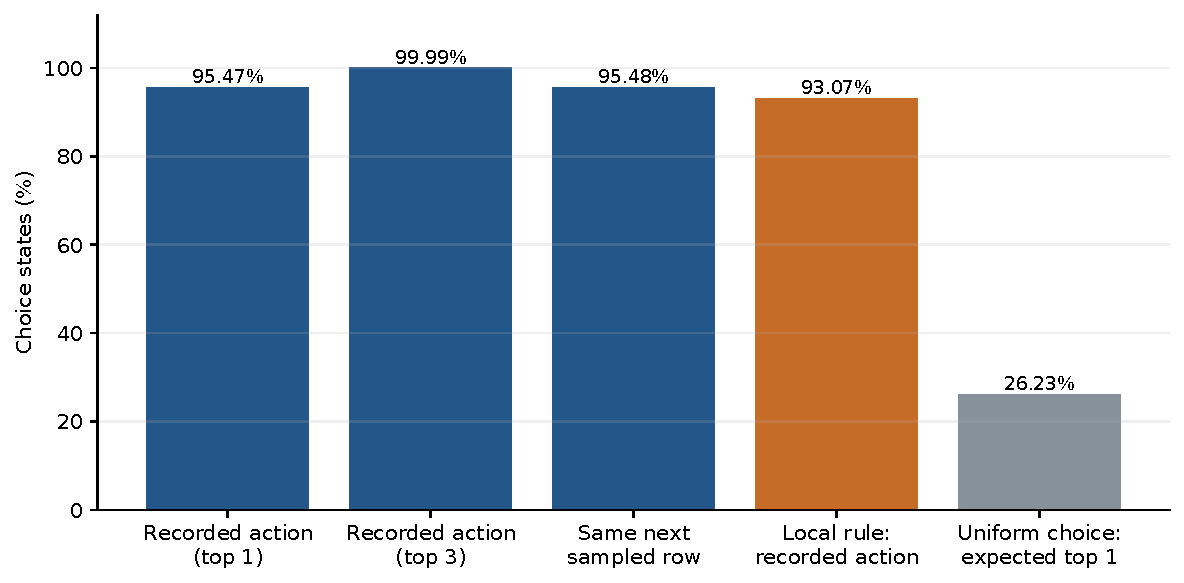
\includegraphics[width=\linewidth]{figures/reduction_action_accuracy.pdf}
 \caption{Next-step comparisons on states with at least two allowed
 actions. The uniform reference assigns equal probability to every
 available action. The tie-averaged result shares credit equally
 among highest-scoring tied actions. The same-row comparison permits different
 identities that produce the same sampled next row.}
 \label{fig:reduction-action-accuracy}
\end{figure}

The model assigns a probability to every supplied action, with
probabilities summing to one. We compare the selected action's
reported probability with observed agreement after grouping
predictions into ten fixed confidence intervals. Let
$\mathcal D^{\rm test}_{\rm choice}$ be the set of held-out states
with at least two allowed actions, and let $a_n^\star$ be the
recorded action at state $n$. Applying the negative logarithmic
loss in Eq.~\eqref{eq:reduction-loss} to this set gives 0.400146.
The calculation replaces probabilities below $10^{-38}$ by
$10^{-38}$ when taking their logarithms.

To compare the full probability distribution with the recorded
choice, we also calculate the multiclass Brier score~\cite{Brier1950},
\begin{equation}
 B_{\rm test}
 =\frac{1}{|\mathcal D^{\rm test}_{\rm choice}|}
 \sum_{n\in\mathcal D^{\rm test}_{\rm choice}}
 \sum_{a\in\mathcal A_n}
 \left[p_\theta(a\mid A^{(n)},\mathcal A_n)
       -\mathbf 1_{a=a_n^\star}\right]^2 .
 \label{eq:reduction-brier}
\end{equation}
Here $\mathcal A_n$ is the supplied action set and
$\mathbf 1_{a=a_n^\star}$ equals one for the recorded action and
zero for every other action. We sum over all actions without
dividing by their number, then give each state equal weight.
The resulting score is 0.250632. The confidence comparison in
Figure~\ref{fig:reduction-confidence} uses the frozen scores without
fitting a correction. A forced action has probability one, so these
ranking and confidence comparisons exclude forced states.

\begin{figure}[htbp]
 \centering
 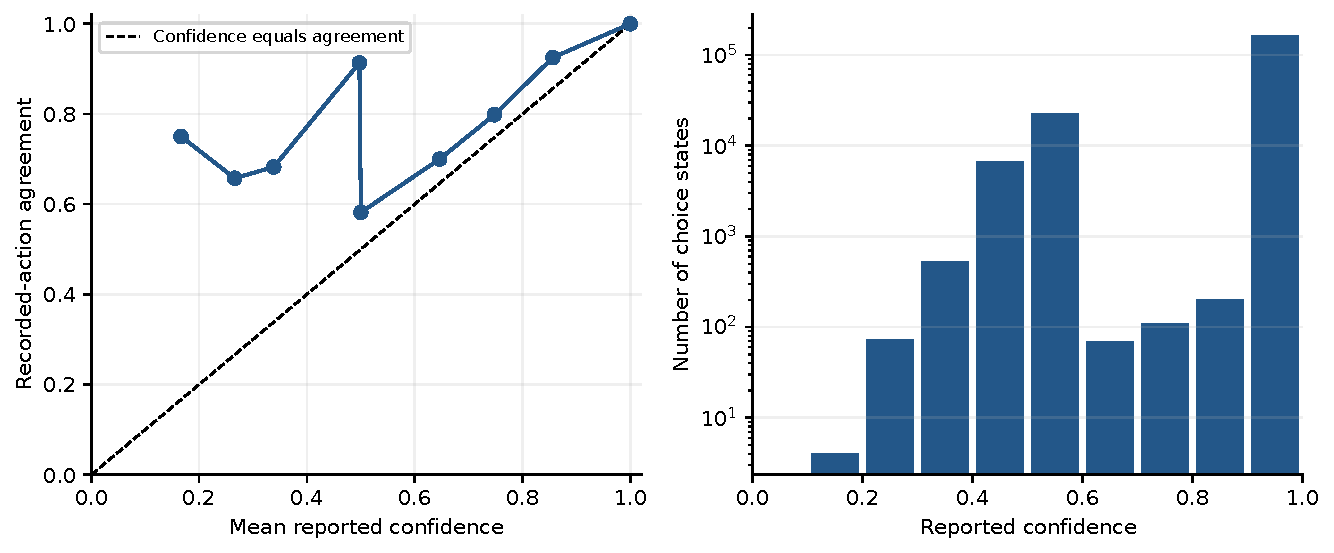
\includegraphics[width=\linewidth]{figures/reduction_confidence.pdf}
 \caption{Reported confidence and recorded-action agreement, with
 the number of choice states in each confidence interval. The
 diagonal represents equality between confidence and agreement.}
 \label{fig:reduction-confidence}
\end{figure}

\begin{figure}[htbp]
 \centering
 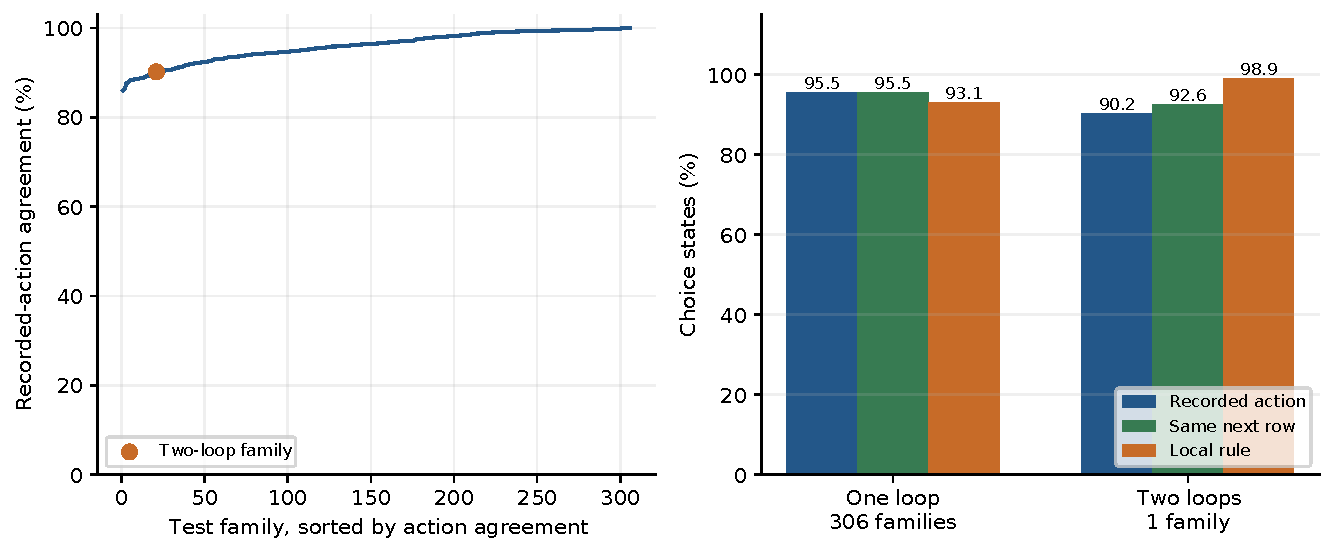
\includegraphics[width=\linewidth]{figures/reduction_families.pdf}
 \caption{Agreement across individual families and loop orders.
 Every higher-loop group uses held-out mass profiles of the
 restricted vacuum families. These comparisons include changes in
 the mathematical family domain as well as loop order.}
 \label{fig:reduction-families}
\end{figure}

\subsection{Complete reductions and arithmetic work}
For complete-path testing, the policy receives the initial target row
and repeatedly selects an allowed identity until the row contains
only protected masters or a stated failure condition occurs.
Decisions use the first finite-field sample. We then replay the
selected sequence at both additional samples and compare the
resulting rows with the exact reference master coefficients
evaluated at those points.

The learned policy matches all three sampled master expansions for
690,302 of 690,382 targets (99.988\%).
The local rule matches all three for 689,700 targets
(99.901\%). The respective numbers without this full
three-sample agreement are 80 and
682. For the learned policy, 77
targets stop when the supplied pool has no allowed identity for the
remaining leading integral, and 3 complete at
the decision sample but fail an additional-sample check. The local
rule gives 664 and 18 in these
two categories. Agreement at the samples is the stated test
criterion; the test does not reconstruct a new symbolic rational
result from the learned path.

\begin{figure}[htbp]
 \centering
 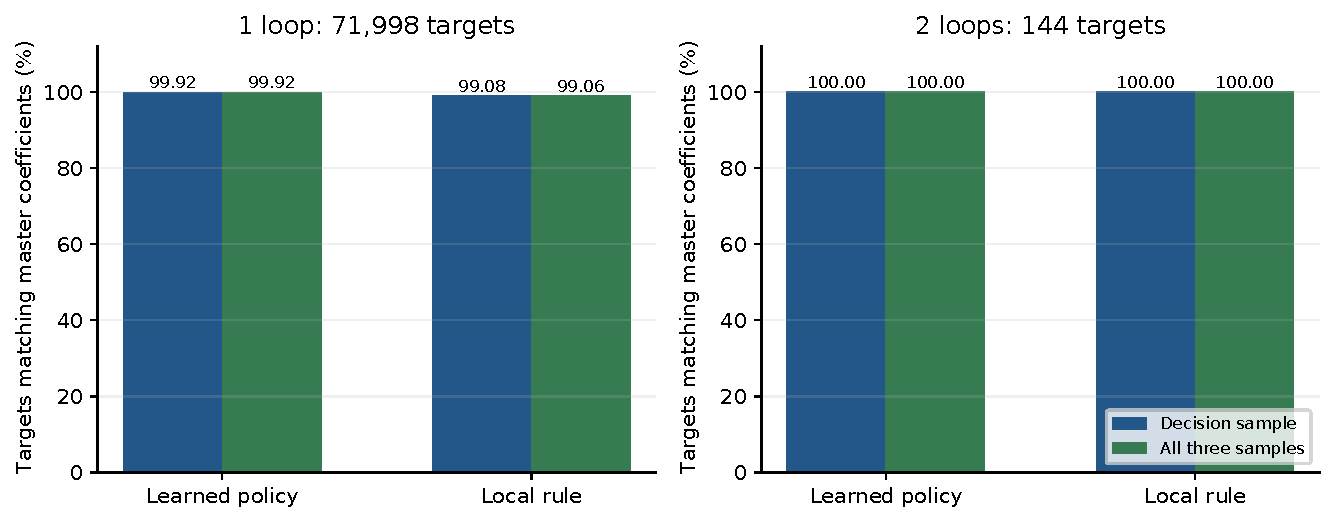
\includegraphics[width=\linewidth]{figures/reduction_rollout_success.pdf}
 \caption{Complete target reductions at each loop order. The left
 panel requires agreement at the decision sample; the right panel
 requires agreement at all three samples.}
 \label{fig:reduction-rollout-success}
\end{figure}

We compare arithmetic counts on the 689,684 targets for which
both policies pass all three samples and the reference count is
nonzero. The learned policy uses fewer committed row operations
than the local rule for 6,846 targets, the same number for
610,196 and more for 72,642. A committed operation changes the
selected target row. Candidate trials used to construct model
features or evaluate the local rule also perform arithmetic, so
Figure~\ref{fig:reduction-operations} shows both accounting choices.
The recorded path supplies a valid reference count without a proof
that this count is minimal.

\begin{figure}[htbp]
 \centering
 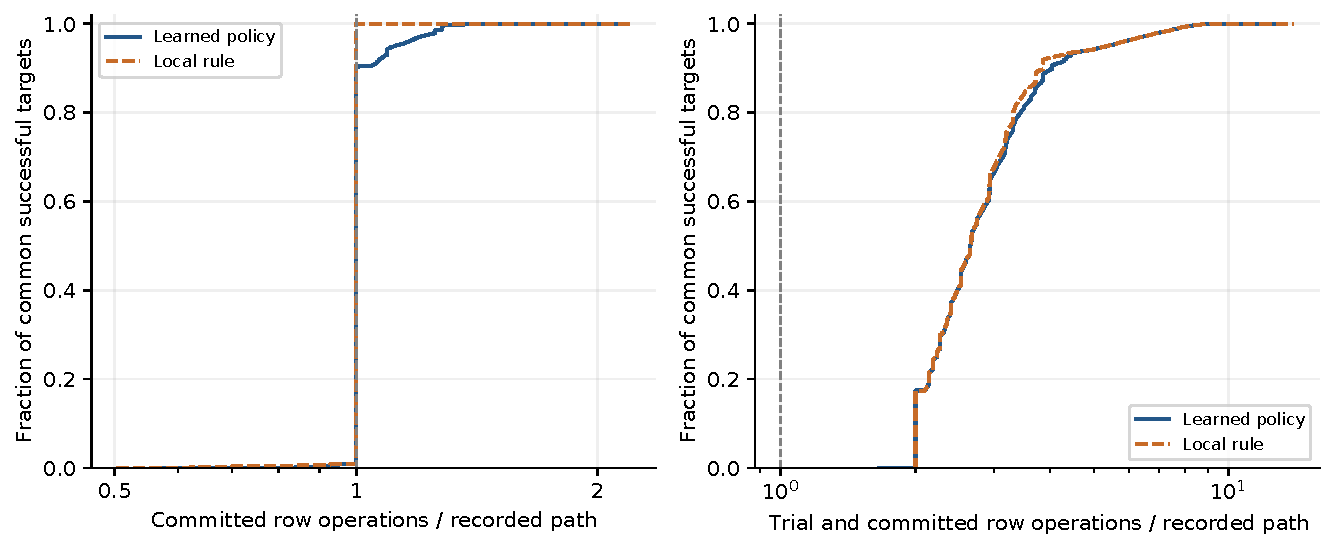
\includegraphics[width=\linewidth]{figures/reduction_operation_counts.pdf}
 \caption{Cumulative distributions of arithmetic counts relative
 to the recorded path, restricted to targets successful for both
 policies. The right panel also includes trial row operations used
 when choosing an action. Both horizontal axes use logarithmic scales.}
 \label{fig:reduction-operations}
\end{figure}

\subsection{Timing, checks and scope}
The mean attempted reduction time is 12.3438 ms per target for
the learned policy and 0.6991 ms for the local rule. The
learned policy therefore takes 17.657 times as long on this
allocation. These times include action selection and committed
elimination within the target-row experiment. We alternate policy
execution order between targets and keep verification and disk
output outside the timed interval. Four CPU workers on the same
compute node process disjoint families, with one computation thread
per worker. Both policies run in the same worker for each target. Figure~\ref{fig:reduction-runtime}
shows the timing distributions on the test allocation.

\begin{figure}[htbp]
 \centering
 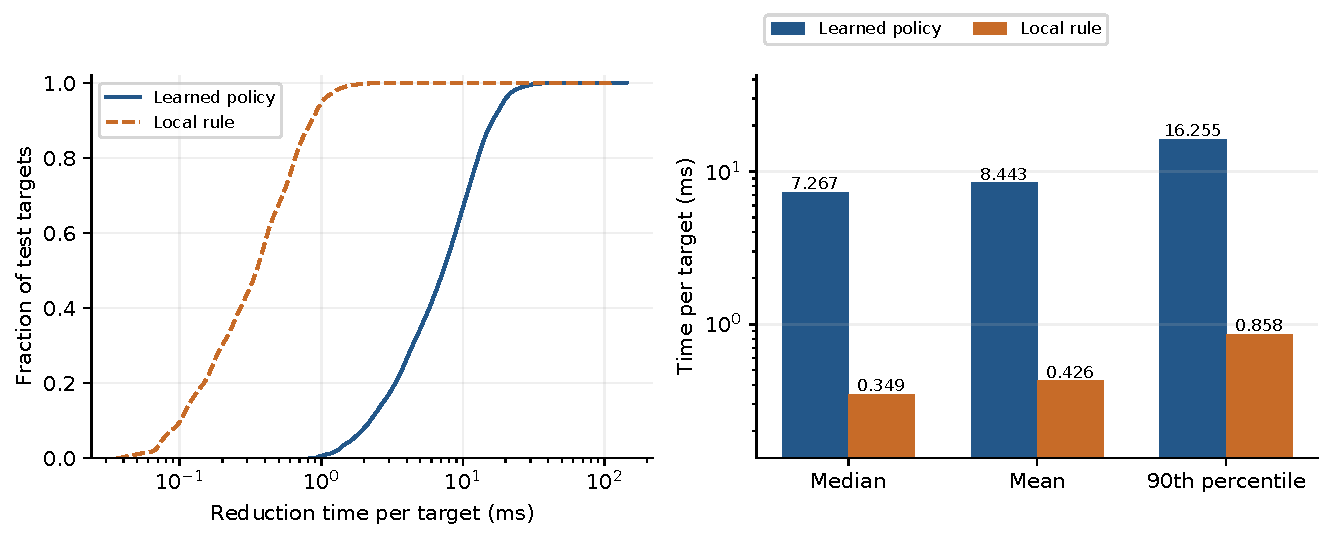
\includegraphics[width=\linewidth]{figures/reduction_runtime.pdf}
 \caption{Attempted target-row reduction times for the learned
 policy and local rule. Both receive identical initial rows,
 source pools and integral ordering.}
 \label{fig:reduction-runtime}
\end{figure}

Independent checks reproduce probability summaries and replay the
committed finite-field operations from the saved paths at the
decision sample. They also
verify the source coefficients, data split and unchanged model hash.
The tests distinguish agreement with a recorded next action from
completion of an allowed alternative path.

The results concern the supplied equation pools and family domains.
Every tested loop order also occurs in training, and related
lower-sector integrals can occur in different mass profiles.
Consequently, the experiment measures held-out profile performance
within these domains. It does not establish globally optimal seed
sets, globally minimal elimination paths or an end-to-end Kira
speedup.
Section~\ref{sec:cost-comparison} then measures complete symbolic reductions with Kira, including model and fallback costs.
\FloatBarrier
